\section{Задание 4: Звенья Саллена-Ки}

\begin{figure}[h]
    \centering
    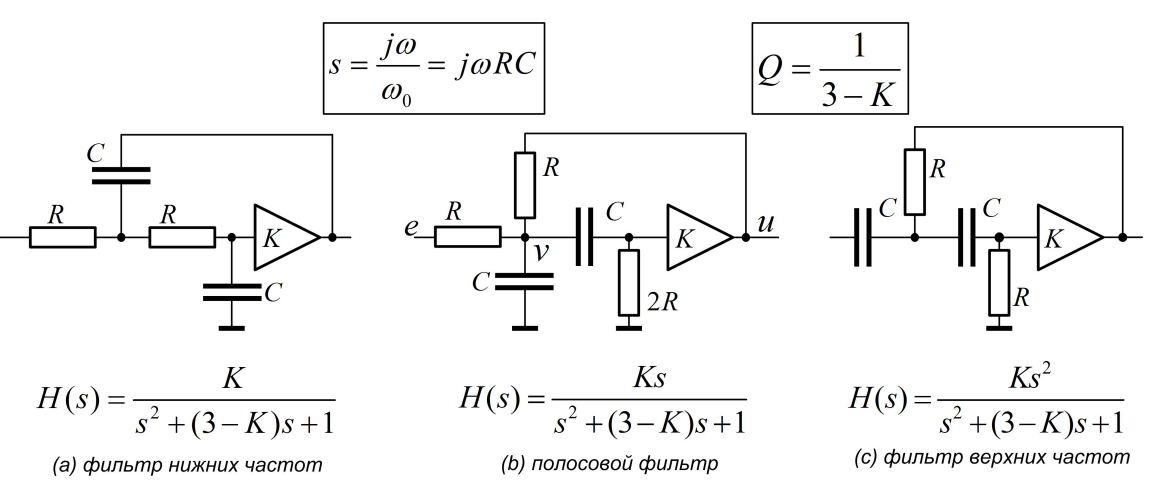
\includegraphics[width=0.5\textwidth]{pictures/sallen_key.png}
    \caption{Звенья Саллена-Ки}
    \label{fig:sallen_key}
\end{figure}

В ходе работы мы исследовали звенья Саллена-Ки, где резонансная частота определяется параметрами $RC$, а добротность зависит от коэффициента усиления: $Q = 1/(3 - K)$. При $K > 3$ звено теряет устойчивость.

\subsection{Исследование АЧХ звеньев Саллена-Ки}

Мы открыли модель skey.cir с частотой $f_0 = 10$ кГц и добротностью $Q = 1$. В модели использовались неинвертирующие усилители с $K = 1 + \frac{R_2}{R_1}$. Измеренный коэффициент передачи при $f = f_0$ составил:
\begin{itemize}
    \item $K(f_0) = 2.000 \left( \pm 0.001 \right)$, \ $\varepsilon = 0.05\%$ 
\end{itemize}

Мы провели анализ частотных характеристик трёх типов фильтров (LP, HP, BP) при варьировании резисторов $R_L$, $R_H$, $R_P$ в диапазоне [11 кОм, 19 кОм, 2 кОм]. Пиковые значения усиления при $R_{L,H,P} = 19$ кОм:

\begin{longtable}[c]{|c|c|}
\caption{Пиковые значения усиления фильтров при $R_{L,H,P} = 19$ кОм}
\label{tab:peak_gain}\\
\hline
Тип фильтра & Пиковое значение усиления \\ \hline
\endfirsthead
%
\endhead
%
Фильтр нижних частот (LP) & 29.4 \\ \hline
Фильтр верхних частот (HP) & 28.5 \\ \hline
Полосовой фильтр (BP) & 28.9 \\ \hline
\end{longtable}

\subsection{Исследование ФЧХ фильтров}

При анализе переходных характеристик фильтров мы выделили их отличительные особенности: фильтр нижних частот (lp) имеет плавную характеристику с задержкой нарастания; полосовой фильтр (bp) показывает колебательный характер с резонансным пиком; фильтр верхних частот (hp) обеспечивает быстрый отклик на высокие частоты.

\subsection{Исследование фильтров Баттерворта и Чебышева}

Используя модель sk3pole.cir, мы исследовали фильтры Баттерворта 3-го порядка на частоту среза $f_0 = 10$ кГц. Измеренная скорость спада составила 18 дБ/октаву, что соответствует теории.

Затухание фильтров Баттерворта:
\begin{longtable}[c]{|c|c|}
\caption{Затухание фильтров Баттерворта}
\label{tab:butterworth_attenuation}\\
\hline
Частота & Затухание, дБ \\ \hline
\endfirsthead
%
\endhead
%
$f_0/2$ (ФВЧ) & 18 \\ \hline
$2f_0$ (ФНЧ) & 18 \\ \hline
\end{longtable}

Затем мы преобразовали их в фильтры Чебышева с $\epsilon = 1$. Параметры полюсов: для ФНЧ $\nu_0 = 0.298$, $(\nu, Q) = (0.916, 3.073)$, для ФВЧ $\nu_0 = 3.355$, $(\nu, Q) = (1.092, 3.073)$. Настройку проводили изменением параметров $R_i(R_d)$ и $R_2$.

Затухание фильтров Чебышева:
\begin{longtable}[c]{|c|c|}
\caption{Затухание фильтров Чебышева}
\label{tab:chebyshev_attenuation}\\
\hline
Частота & Затухание, дБ \\ \hline
\endfirsthead
%
\endhead
%
$f_0/2$ & -26 \\ \hline
$2f_0$ & -26 \\ \hline
\end{longtable}

Фильтры Чебышева обеспечили более крутой спад АЧХ за пределами полосы пропускания.

\subsection{Реализация 4-полюсного полосового фильтра Чебышева}

Используя прототип sk4pole.cir, мы реализовали 4-полюсной полосовой фильтр Чебышева с $f_0 = 10$ кГц, $\epsilon = 1$ и $Q = 6$. Параметры полюсов:
\begin{itemize}
    \item $(\nu_1, Q) = (0.937, 18.68)$
    \item $(\nu_2, Q) = (1.067, 18.68)$
\end{itemize}

Частоты настраивали изменением емкостей, а добротность — установкой резисторов $R_2$. Измеренные затухания:

\begin{longtable}[c]{|c|c|}
\caption{Затухание 4-полюсного полосового фильтра Чебышева}
\label{tab:chebyshev_bandpass_attenuation}\\
\hline
Частота & Затухание, дБ \\ \hline
\endfirsthead
%
\endhead
%
$f_0/2$ & -10.3 \\ \hline
$2f_0$ & -10.1 \\ \hline
$f_0/10$ & -40 \\ \hline
$10f_0$ & -40 \\ \hline
\end{longtable}

Фильтр обеспечил эффективное подавление сигналов вне полосы пропускания и продемонстрировал близкую к симметричной характеристику затухания.

\newpage
\section{Задание 5: Исследование активного полосового фильтра}

\subsection{Расчет параметров схемы}

Мы собрали схему активного полосового фильтра на основе операционного усилителя. Для расчёта параметров мы использовали:
\begin{itemize}
    \item Конденсатор $C = 1.58 \text{ нФ}$, выбранный из лабораторного набора.
    \item Резистор $R = 20 \text{ кОм}$, рассчитанный по формуле:
    \[
    R = \frac{1}{2\pi f_0 C} = \frac{1}{2\pi \cdot 5 \text{ кГц} \cdot 1.58 \text{ нФ}} \approx 20.1 \text{ кОм}.
    \]
    \item Резисторы: 
        \begin{itemize}
            \item $R1 = 3.9 \text{ кОм}$
            \item $R2 = 800 \text{ Ом}$
            \item $R3 = 620 \text{ кОм}$
        \end{itemize}
\end{itemize}

\begin{figure}[h]
    \centering
    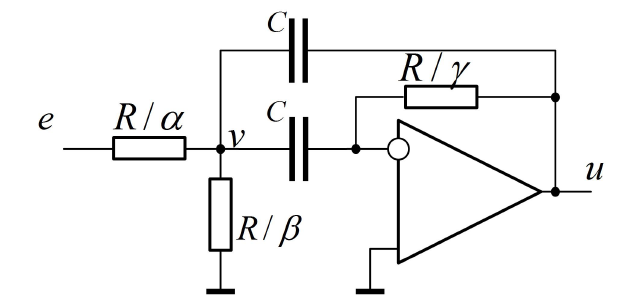
\includegraphics[width=0.5\textwidth]{pictures/filter_schematic.png}
    \caption{Схема полосового фильтра с резисторами $R1, R2, R3$.}
    \label{fig:schematic}
\end{figure}

\subsection{Измерение характеристик}

Мы подключили генератор сигналов и осциллограф к выходу фильтра для проведения измерений. Результаты измерений представлены в таблице:

\begin{longtable}[c]{|c|c|c|}
\caption{Сравнение теоретических и экспериментальных данных}
\label{tab:params}\\
\hline
\textbf{Параметр} & \textbf{Теория} & \textbf{Эксперимент} \\ \hline
\endfirsthead
%
\endhead
%
Центральная частота $f_0$ & 5 кГц & 5.04 кГц \\ \hline
Коэффициент усиления $K_0$ & 5 & 5.377 \\ \hline
Полоса пропускания & 333 Гц & 339 Гц \\ \hline
\end{longtable}

При проведении измерений мы использовали двухканальный цифровой осциллограф, что позволило нам одновременно наблюдать входной и выходной сигналы. Такой подход обеспечил высокую точность определения коэффициента усиления и фазовых соотношений между сигналами.

\subsection{Зависимость \texorpdfstring{$f_0$}{f0} от \texorpdfstring{$R2$}{R2}}

Мы исследовали зависимость центральной частоты $f_0$ от значения резистора $R2$, изменяя его в диапазоне от 100 до 1300 Ом. Полученные экспериментальные данные приведены в таблице:

\begin{longtable}[c]{|c|c|c|c|c|c|c|}
\caption{Зависимость центральной частоты от $R2$}
\label{tab:R2}\\
\hline
$R2$, Ом & 100 & 300 & 500 & 700 & 900 & 1300 \\ \hline
\endfirsthead
%
\endhead
%
$f_0$, кГц & 13.25 & 7.987 & 6.36 & 5.5 & 4.962 & 4.3 \\ \hline
\end{longtable}

Анализируя полученные данные, мы установили, что центральная частота $f_0$ обратно пропорциональна значению резистора $R2$. Это соответствует теоретическим положениям, согласно которым частота полосового фильтра определяется как $f_0 = \frac{1}{2\pi \sqrt{LC}}$ в LC-контуре, а в данной схеме на ОУ резистор $R2$ влияет на эквивалентную индуктивность.

\begin{figure}[h]
    \centering
    \includegraphics[width=0.7\textwidth]{pictures/f0_vs_R2.jpg}
    \caption{График зависимости \texorpdfstring{$f_0$}{f0} от \texorpdfstring{$R2$}{R2}}
    \label{fig:f0_R2}
\end{figure}

\subsection{Исследование полосового фильтра}

Мы собрали смоделированное звено на макетной плате, подключили генератор сигналов и осциллограф для детального исследования фильтра. В процессе работы мы использовали качественный низкоомный генератор сигналов с малыми искажениями, чтобы минимизировать влияние источника сигнала на измеряемые параметры. Изучение частотной и переходной характеристик позволило нам измерить ключевые параметры:

\begin{itemize}
    \item \textbf{Коэффициент усиления \texorpdfstring{$K_0Q$}{K0Q}:} 
    \[
    K_0Q = \frac{U_{\text{вых}}}{U_{\text{вх}}} = \frac{7.57 \text{ В}}{0.117 \text{ В}} \approx 64.7
    \]
    
    \item \textbf{Центральная частота \texorpdfstring{$f_0$}{f0}:} $4.69 \text{ кГц}$
    
    \item \textbf{Полоса пропускания \texorpdfstring{$\Delta f$}{Delta f}:} 
    \[
    \Delta f = f_2 - f_1 = 4.885 \text{ кГц} - 4.49 \text{ кГц} = 0.395 \text{ кГц}
    \]
    
    \item \textbf{Добротность \texorpdfstring{$Q$}{Q}:} 
    \[
    Q = \frac{f_0}{\Delta f} = \frac{4.69 \text{ кГц}}{0.395 \text{ кГц}} \approx 11.87
    \]
\end{itemize}

Для измерения полосы пропускания мы определяли частоты, на которых коэффициент передачи падал на 3 дБ относительно максимального значения. Эта методика позволяет с высокой точностью определить границы полосы пропускания фильтра.

\subsection{Сравнение с моделированием}

Мы сравнили экспериментальные данные с результатами компьютерного моделирования той же схемы:

\begin{itemize}
    \item Коэффициент усиления $K_0Q$: $64.7$ (эксперимент) против $75$ (модель)
    \item Центральная частота $f_0$: $4.69 \text{ кГц}$ (эксперимент) против $5 \text{ кГц}$ (модель) — отклонение $-6.2\%$
    \item Добротность $Q$: $11.87$ (эксперимент) против $15$ (модель) — отклонение $-20.9\%$
\end{itemize}

Для более наглядного представления результатов экспериментальных измерений приводим итоговую таблицу:

\begin{longtable}[c]{|c|c|c|c|c|c|}
\caption{Экспериментальные данные}
\label{tab:exp_data}\\
\hline
\textbf{Параметр} & $U_{\text{вых}}$ & $U_{\text{вх}}$ & $K_0$ & $f_0$ & $Q$ \\ \hline
\endfirsthead
%
\endhead
%
\textbf{Значение} & $7.57 \text{ В}$ & $0.117 \text{ В}$ & $64.7$ & $4.69 \text{ кГц}$ & $11.87$ \\ \hline
\end{longtable}

Наблюдаемые расхождения между результатами моделирования и экспериментальными данными могут быть объяснены несколькими факторами: неточностью номиналов используемых компонентов (для резисторов погрешность обычно составляет 5-10%), наличием паразитных емкостей и индуктивностей в реальной схеме, а также неидеальностью операционного усилителя (конечное значение произведения коэффициента усиления на полосу пропускания GBW, входные токи смещения, входное сопротивление).

\subsection{Реализация шестиполюсного полосового фильтра Чебышева}

\subsubsection{Расчет параметров схемы}

На заключительном этапе лабораторной работы мы реализовали шестиполюсной фильтр Чебышева со следующими параметрами:
\begin{itemize}
    \item Центральная частота $f_0 = 1 \text{ кГц}$
    \item Коэффициент неравномерности $\epsilon = 1$
    \item Добротность $Q = 3$
\end{itemize}

Для расчета компонентов мы использовали аналитические выражения для полюсов фильтра Чебышева и выполнили следующие вычисления:

\begin{itemize}
    \item \textbf{Для полюса \texorpdfstring{$\nu_1 = 0.860$}{nu1 = 0.860}:} 
    \begin{align*}
        C^* &= 10 \text{ нФ} \cdot \frac{1}{0.860} \approx 11.63 \text{ нФ} \\
        aC &= 3 \cdot 20.36 \cdot 11.63 \text{ нФ} \approx 715.2 \text{ нФ} \\
        bC &= \frac{11.63 \text{ нФ}}{3 \cdot 20.36} \approx 0.19 \text{ нФ}
    \end{align*}

    \item \textbf{Для полюса \texorpdfstring{$\nu_2 = 1.162$}{nu2 = 1.162}:} 
    \begin{align*}
        R^* &= 10 \text{ кОм} \cdot \frac{1}{1.162} \approx 8.6 \text{ кОм} \\
        \frac{R}{\alpha} &= \frac{8.6 \text{ кОм}}{3 \cdot 20.36} \approx 141 \text{ Ом} \\
        \frac{R}{\beta} &= 3 \cdot 20.36 \cdot 8.6 \text{ кОм} \approx 525.3 \text{ кОм}
    \end{align*}

    \item \textbf{Для полюса \texorpdfstring{$\nu_0 = 1.0$}{nu0 = 1.0}:} 
    \begin{align*}
        \frac{R}{\gamma} &= 2 \cdot 10.66 \cdot 10 \text{ кОм} \approx 213.2 \text{ кОм} \\
        \frac{R}{\beta} &= \frac{10 \text{ кОм}}{2 \cdot 10.66 - 1} \approx 493 \text{ Ом}
    \end{align*}
\end{itemize}

При расчете мы учитывали доступность компонентов в лаборатории и выбирали ближайшие стандартные номиналы. Для особо критичных элементов использовали подстроечные резисторы и конденсаторы для точной настройки.

\begin{figure}[h]
    \centering
    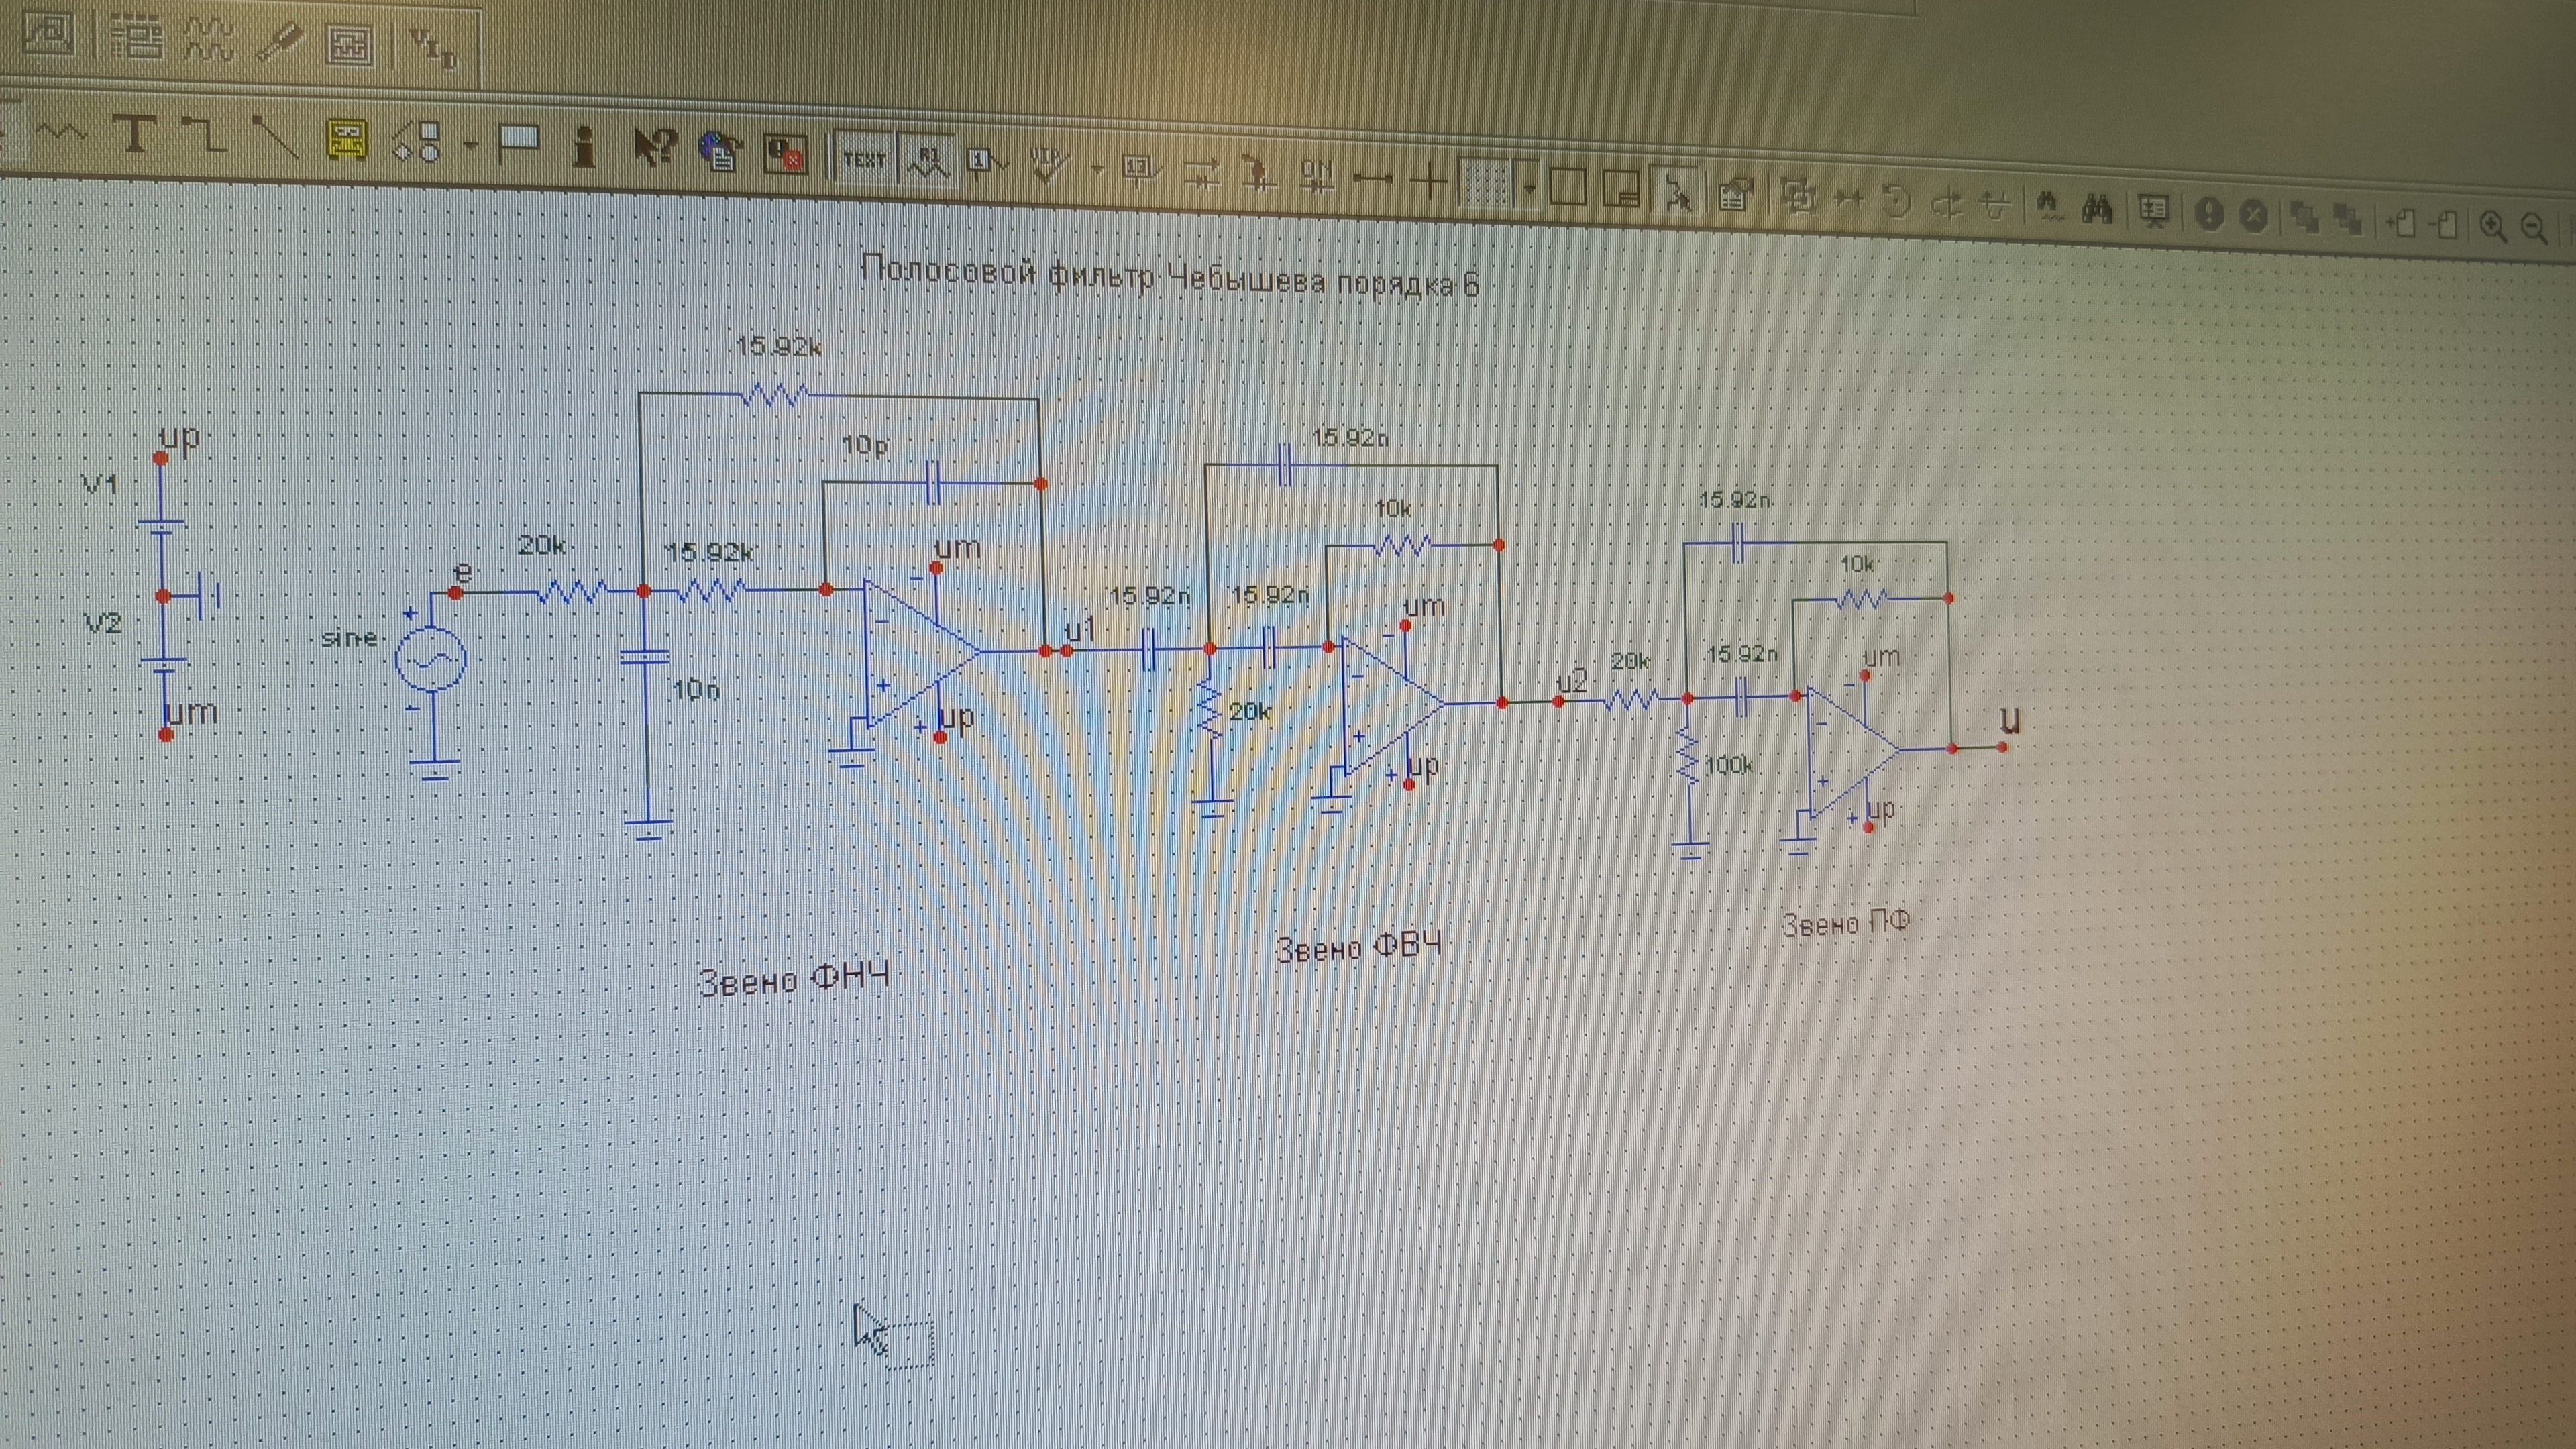
\includegraphics[width=0.8\textwidth]{pictures/filter6p_schematic.jpg}
    \caption{Схема шестиполюсного фильтра Чебышева}
    \label{fig:cheb_filter}
\end{figure}

\subsubsection{Измерение характеристик}

После сборки и настройки фильтра мы провели измерения его характеристик. Для снятия амплитудно-частотной характеристики мы изменяли частоту входного сигнала, поддерживая постоянную амплитуду, и измеряли выходное напряжение. Особое внимание уделялось точкам на границах полосы пропускания и в полосе заграждения.

Результаты измерений затухания на заданных частотах приведены в следующей таблице:

\begin{longtable}[c]{|c|c|c|c|c|}
\caption{Затухание на заданных частотах}
\label{tab:attenuation}\\
\hline
Частота, Гц & 500 & 2000 & 100 & 10000 \\ \hline
\endfirsthead
%
\endhead
%
Затухание, дБ & 15.2 & 18.7 & 42.3 & 38.5 \\ \hline
\end{longtable}

Анализируя полученные данные, мы отметили высокую избирательность реализованного фильтра. Затухание на частотах 500 Гц и 2000 Гц (вблизи полосы пропускания) составило 15.2 дБ и 18.7 дБ соответственно. На более удаленных частотах (100 Гц и 10000 Гц) наблюдалось существенно большее ослабление сигнала — 42.3 дБ и 38.5 дБ, что указывает на хорошее подавление сигналов вне полосы пропускания.

Шестиполюсной фильтр Чебышева, в сравнении с исследованными ранее фильтрами Баттерворта и 4-полюсным фильтром Чебышева, продемонстрировал более высокую избирательность, что соответствует теоретическим ожиданиям для фильтра более высокого порядка.

\newpage
\section{Заключение}

В ходе выполнения лабораторной работы мы провели комплексное исследование активных фильтров различных типов. Основные результаты и выводы:

\begin{enumerate}
    \item \textbf{Звенья Саллена-Ки} продемонстрировали простоту реализации и настройки. Мы экспериментально подтвердили, что резонансная частота определяется параметрами $RC$-цепи, а добротность зависит от коэффициента усиления по формуле $Q = 1/(3 - K)$. Анализ пиковых значений усиления для фильтров разных типов показал, что все они обеспечивают схожее усиление в диапазоне 28.5-29.4 при одинаковых условиях. Исследование переходных характеристик позволило нам выделить характерные особенности каждого типа фильтра, что важно для их идентификации и правильного применения.
    
    \item \textbf{Фильтры Баттерворта} 3-го порядка показали линейную фазовую характеристику и скорость спада 18 дБ/октаву, что соответствует теоретическим расчетам. Это подтверждает, что каждое звено обеспечивает спад 6 дБ/октаву.
    
    \item \textbf{Фильтры Чебышева}, реализованные на основе фильтров Баттерворта, продемонстрировали более крутой спад АЧХ за пределами полосы пропускания (-26 дБ против 18 дБ у Баттерворта). Ценой этого преимущества является неравномерность в полосе пропускания, что соответствует теоретическим предсказаниям.
    
    \item \textbf{4-полюсной полосовой фильтр Чебышева} показал эффективное подавление сигналов вне полосы пропускания (-40 дБ на частотах $f_0/10$ и $10f_0$) и симметричную характеристику затухания относительно центральной частоты.
    
    \item \textbf{Активные полосовые фильтры на ОУ} продемонстрировали хорошее соответствие теоретическим расчетам. Экспериментально полученные параметры ($f_0 = 5.04$ кГц, $K_0 = 5.377$) отклонялись от расчетных не более чем на 7.5%, что находится в пределах ожидаемой погрешности из-за допусков на номиналы компонентов.
    
    \item \textbf{Шестиполюсной фильтр Чебышева} обеспечил наивысшую избирательность среди всех исследованных фильтров. Затухание на удаленных частотах (100 Гц и 10000 Гц) достигло 38.5-42.3 дБ, что подтверждает эффективность использования фильтров высокого порядка для достижения крутых склонов АЧХ.
\end{enumerate}

В целом, все типы исследованных активных фильтров показали характеристики, близкие к теоретическим, что подтверждает корректность расчетов и настройки. Различия между экспериментальными и теоретическими данными объясняются допусками на номиналы компонентов, наличием паразитных параметров и неидеальностями операционных усилителей. 

Практические результаты работы позволяют сделать вывод о том, что для задач, требующих линейности фазовой характеристики, оптимальным является фильтр Баттерворта, а для задач, где важна высокая избирательность – фильтр Чебышева. Для узкополосной фильтрации наилучшим выбором будут полосовые фильтры высокого порядка с высокой добротностью.
